% 编译方式：请使用 XeLaTeX 编译（本文档使用了 ctex 宏包以支持中文）。
\documentclass[12pt,a4paper]{ctexart}

\usepackage{amsmath, amssymb}
\usepackage{amsthm}
\usepackage{geometry}
\geometry{margin=2.5cm}
\usepackage{booktabs}
\usepackage{graphicx}

\title{\bfseries 数值分析实验报告：雅可比迭代法求解线性方程组}
\author{（姓名）\quad （学号）}
\date{\today}

\begin{document}
\maketitle

\section{问题描述与矩阵构造}

考虑线性方程组
\begin{equation}
  Ax = b,
\end{equation}
其中系数矩阵取下面的 $5\times 5$ \textbf{严格对角占优}矩阵
\begin{equation}
  A =
  \begin{pmatrix}
    10 & 1 & -1 & 2 & 0 \\
    1 & 12 & 3 & -1 & 1 \\
    -2 & 1 & 15 & 2 & -3 \\
    1 & -2 & 1 & 11 & 2 \\
    0 & 2 & -1 & 3 & 13
  \end{pmatrix}.
\end{equation}
右端向量取为
\begin{equation}
  b = A\,(1,2,3,4,5)^{\top} = (17,\,35,\,38,\,54,\,78)^{\top},
\end{equation}
因此方程组的\textbf{精确解}为 $x^{\ast} = (1,2,3,4,5)^{\top}$。

逐行验证严格对角占优条件 $|a_{ii}| > \sum_{j\neq i}|a_{ij}|$：
\begin{equation*}
  \begin{aligned}
    \text{第 }0\text{ 行：}& 10 > 1+1+2+0 = 4,\\
    \text{第 }1\text{ 行：}& 12 > 1+3+1+1 = 6,\\
    \text{第 }2\text{ 行：}& 15 > 2+1+2+3 = 8,\\
    \text{第 }3\text{ 行：}& 11 > 1+2+1+2 = 6,\\
    \text{第 }4\text{ 行：}& 13 > 0+2+1+3 = 6,
  \end{aligned}
\end{equation*}
每一行均严格成立，故 $A$ 严格对角占优。这一性质（而非任意的 $A$）正是保证下面
雅可比迭代\textbf{收敛}的关键。

\section{雅可比迭代法的数学推导}

将系数矩阵分裂为
\begin{equation}
  A = D + L + U,
\end{equation}
其中 $D=\operatorname{diag}(a_{11},\dots,a_{nn})$ 为对角部分，$L$ 为严格下三角部分，
$U$ 为严格上三角部分（对角线均为 $0$）。则方程组等价于
\begin{equation}
  D x = b - (L+U)\,x
  \quad\Longleftrightarrow\quad
  x = D^{-1}\bigl(b - (L+U)\,x\bigr).
\end{equation}
把上式右端的 $x$ 取为上一次迭代的近似值，即得到\textbf{雅可比迭代}：
\begin{equation}
  x^{(k+1)} = D^{-1}\bigl(b - (L+U)\,x^{(k)}\bigr),\qquad k=0,1,2,\dots
\end{equation}
写成逐分量形式（由 $D$ 是对角阵，$D^{-1}$ 即对各分量除以 $a_{ii}$）：
\begin{equation}
  \boxed{\;
  x_i^{(k+1)} = \frac{1}{a_{ii}}\Bigl( b_i - \sum_{j\neq i} a_{ij}\, x_j^{(k)} \Bigr),
  \qquad i = 1,2,\dots,n.
  \;}
\end{equation}
这正是任务书给出的迭代公式。记迭代矩阵
\begin{equation}
  B = -D^{-1}(L+U) = D^{-1}(D - A) = I - D^{-1}A,
  \qquad
  c = D^{-1}b,
\end{equation}
则迭代可写为紧凑的线性迭代形式
\begin{equation}
  x^{(k+1)} = B\, x^{(k)} + c.
\end{equation}
若 $x^{\ast}$ 是精确解，则 $x^{\ast} = B x^{\ast} + c$；相减得到误差向量
$e^{(k)} = x^{(k)} - x^{\ast}$ 的递推关系
\begin{equation}
  e^{(k+1)} = B\, e^{(k)}
  \quad\Longrightarrow\quad
  e^{(k)} = B^{k}\, e^{(0)}.
\end{equation}

\section{严格对角占优矩阵的收敛性证明}

\textbf{定理}（严格对角占优下雅可比迭代的收敛性）。设 $A\in\mathbb R^{n\times n}$
严格对角占优，即对每个 $i$ 有
\begin{equation}
  |a_{ii}| > \sum_{j\neq i} |a_{ij}|,
\end{equation}
则雅可比迭代对任意初值 $x^{(0)}$ 收敛到唯一解 $x^{\ast}$。

\begin{proof}
  迭代矩阵 $B = D^{-1}(D-A)$ 的元素为
  \begin{equation}
    B_{ii} = 0,\qquad
    B_{ij} = -\frac{a_{ij}}{a_{ii}}\quad (j\neq i).
  \end{equation}
  因此第 $i$ 行的绝对值之和为
  \begin{equation}
    \sum_{j=1}^{n} |B_{ij}|
    = \sum_{j\neq i} \frac{|a_{ij}|}{|a_{ii}|}
    = \frac{1}{|a_{ii}|}\sum_{j\neq i} |a_{ij}| < 1,
  \end{equation}
  其中最后一步严格不等式正是严格对角占优条件。于是矩阵的无穷范数满足
  \begin{equation}
    \|B\|_{\infty}
    = \max_{1\le i\le n}\sum_{j=1}^{n}|B_{ij}| < 1.
  \end{equation}
  对任意矩阵范数 $\|\cdot\|$ 及其诱导范数，谱半径满足 $\rho(B) \le \|B\|_{\infty}$，
  故
  \begin{equation}
    \rho(B) \le \|B\|_{\infty} < 1.
  \end{equation}
  由 $e^{(k)} = B^{k}e^{(0)}$ 与 $\rho(B)<1$ 知 $\lim_{k\to\infty}B^{k}=0$，于是
  $e^{(k)}\to 0$，即 $x^{(k)}\to x^{\ast}$。又由 $\rho(B)<1$ 知 $I-B$ 非奇异，
  方程 $x^{\ast}=B x^{\ast}+c$ 即 $(I-B)x^{\ast}=c$ 有唯一解，从而该解正是
  $Ax=b$ 的唯一解。\qedhere
\end{proof}

此外，利用不等式
\begin{equation}
  \|e^{(k)}\|_{\infty} \le \|B\|_{\infty}^{k}\,\|e^{(0)}\|_{\infty},
\end{equation}
可给出\textbf{先验}的线性收敛速率估计：误差每迭代一步至少按因子
$\|B\|_{\infty}<1$ 缩小。这一经典收敛理论详见 Varga~\cite{varga2000} 与
Golub--Van~Loan~\cite{golub2013}。

\section{本次实验的收敛速度分析}

对本实验的矩阵 $A$，对角部分为
$D=\operatorname{diag}(10,12,15,11,13)$，迭代矩阵 $B = D^{-1}(D-A)$ 的无穷范数为
\begin{equation}
  \|B\|_{\infty} = \max_{i}\frac{1}{|a_{ii}|}\sum_{j\neq i}|a_{ij}| = \frac{6}{11} \approx 0.5455 < 1,
\end{equation}
最大值取自第 $3$ 行（$(1+2+1+2)/11 = 6/11$）。这从先验上保证了迭代收敛。

进一步计算迭代矩阵的\textbf{谱半径}
\begin{equation}
  \rho(B) = \max_{i}|\lambda_i(B)| \approx 0.4964 < 1,
\end{equation}
谱半径 $\rho(B)$ 才是渐近意义下每次迭代误差的缩减因子。由于
$\rho(B) \approx 0.4964 \approx 0.5$，误差每迭代一步约缩小一半，呈现典型的
\textbf{一阶（线性）收敛}。

数值实验的结果与理论完全吻合：
\begin{itemize}
  \item 初值取 $x^{(0)}=(0,0,0,0,0)^{\top}$，容差 $\mathrm{tol}=10^{-6}$，最大迭代
    次数 $1000$；
  \item 仅用 $k=19$ 次迭代即满足停止条件
    $\|x^{(19)}-x^{(18)}\|_{\infty} = 7.483\times10^{-7} < 10^{-6}$；
  \item 由初始误差尺度（$\|x^{(1)}-x^{(0)}\|_{\infty}=6.0$）到 $10^{-6}$ 量级，
    按谱半径估算所需迭代次数为
    \begin{equation}
      k \approx \frac{\ln(10^{-6}/6)}{\ln(0.4964)} \approx 22,
    \end{equation}
    与实测的 $19$ 次在量级上一致——早期迭代中误差的高频分量（对应模更小的特征值）
    衰减更快，故实际收敛略快于谱半径给出的最坏情形估计。
  \item 相邻迭代误差比 $\|x^{(k+1)}-x^{(k)}\|_{\infty}/\|x^{(k)}-x^{(k-1)}\|_{\infty}$
    随 $k$ 增大逐渐趋向 $\rho(B)\approx 0.4964$，印证了“谱半径是渐近收敛速率”的结论。
\end{itemize}

收敛曲线（半对数坐标）如图~\ref{fig:conv} 所示，误差随迭代次数呈近似直线下降，
这正是线性收敛在对数坐标下的典型特征。

\begin{figure}[htbp]
  \centering
  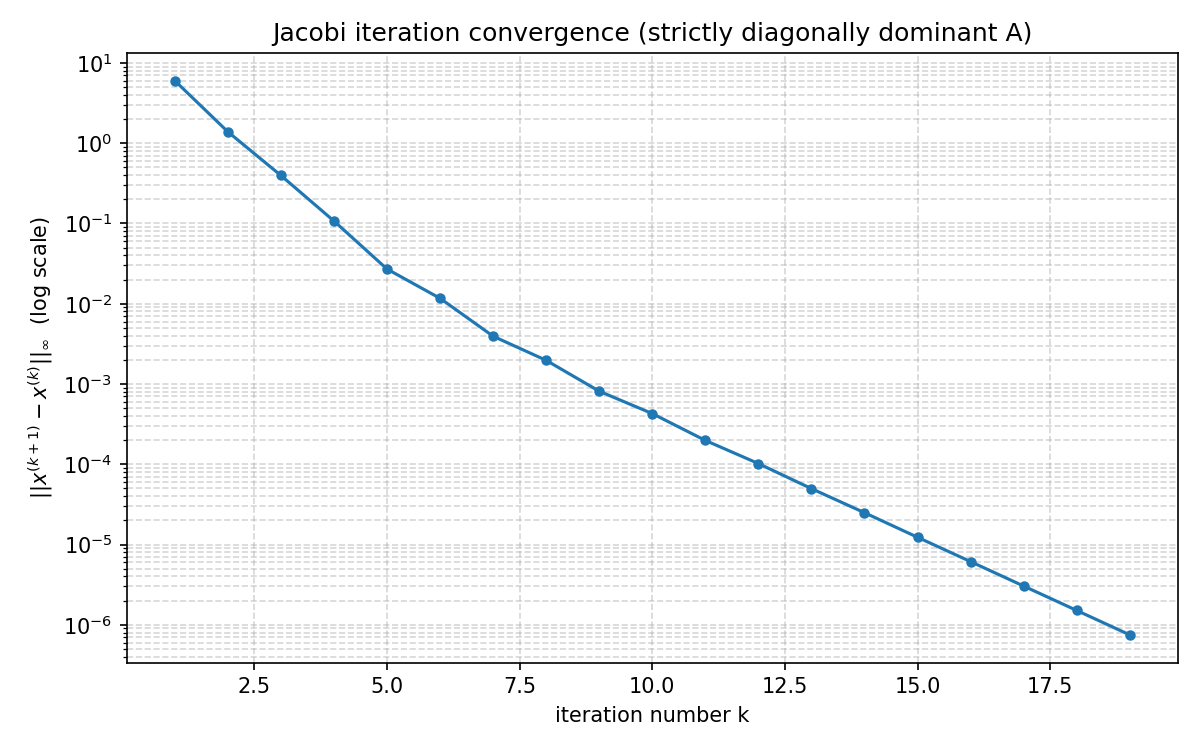
\includegraphics[width=0.72\textwidth]{jacobi_convergence.png}
  \caption{雅可比迭代收敛曲线（半对数坐标）}
  \label{fig:conv}
\end{figure}

\section{与直接法 \texttt{numpy.linalg.solve} 的对比结论}

迭代结束后，用直接法 \verb|numpy.linalg.solve|（内部为带部分主元的 LU 分解）求得的
参考解与雅可比迭代解分别为
\begin{equation*}
  x_{\text{jacobi}} = (0.999999,\,2.000001,\,2.999999,\,4.000001,\,4.999999)^{\top},
  \qquad
  x_{\text{ref}} = (1,\,2,\,3,\,4,\,5)^{\top},
\end{equation*}
相对误差（$2$-范数）为
\begin{equation}
  \frac{\|x_{\text{jacobi}} - x_{\text{ref}}\|_2}{\|x_{\text{ref}}\|_2}
  \approx 2.058\times 10^{-7}.
\end{equation}
对比两种方法的结论如下：

\begin{enumerate}
  \item \textbf{收敛性与稳定性}：直接法（LU 分解/消元）在有限步内给出结果，对
    本实验这种良态问题精度达到机器精度量级；雅可比迭代法则以
    $\rho(B)\approx 0.4964$ 的线性速率逐步逼近，达到同样精度需要约 $20$ 次迭代。
  \item \textbf{适用条件}：直接法对一般可逆矩阵均可用（配合部分主元法对几乎所有
    矩阵稳定）；而雅可比迭代法\textbf{不保证}对所有矩阵收敛，仅当谱半径
    $\rho(B)<1$ 时收敛。严格对角占优矩阵恰是保证 $\rho(B)\le\|B\|_{\infty}<1$ 的
    充分条件，这也是本实验特意构造严格对角占优矩阵的原因。
  \item \textbf{计算量}：直接法求解 $n$ 阶方程组需 $O(n^3)$ 次运算；雅可比迭代
    每次迭代仅需一次矩阵—向量乘，$O(n^2)$ 次运算，若迭代次数远小于 $n$ 则有优势。
  \item \textbf{大规模与稀疏问题}：当 $A$ 是大型稀疏矩阵（例如来自偏微分方程离散化
    的矩阵）时，直接法会因填充（fill-in）而丧失稀疏性、内存与时间代价高昂，此时
    迭代法（雅可比、Gauss--Seidel、共轭梯度等）成为主流选择~\cite{saad2003}。本实验中 $5\times 5$
    的小矩阵用直接法更快，但雅可比迭代展示了迭代法求解的思想与收敛机理。
\end{enumerate}

值得一提的是，针对雅可比迭代收敛较慢的问题，已有多种改进与加速方案：例如
Milaszewicz~\cite{milaszewicz1987} 提出了改进的雅可比/高斯--赛德尔迭代；
Pratapa 等~\cite{pratapa2015} 将 Anderson 加速引入雅可比迭代，用于高效求解
大规模稀疏线性方程组。

\section{加速方法对比实验}

在标准雅可比迭代（$19$ 次迭代、谱半径 $\rho(B_J)\approx0.4964$）的基础上，本实验
在\textbf{同一矩阵}、\textbf{同一初值} $x^{(0)}=0$、\textbf{同一容差}
$\mathrm{tol}=10^{-6}$ 下，对比了四种加速方法。各方法均写成
$x^{(k+1)}=B x^{(k)}+c$ 的线性迭代形式：

\paragraph{阻尼雅可比（Damped Jacobi）。}引入松弛参数 $\omega$，对本次雅可比
修正按比例加权：
\begin{equation}
  x^{(k+1)} = (1-\omega)\,x^{(k)} + \omega\, D^{-1}\bigl(b-(L+U)\,x^{(k)}\bigr),
\end{equation}
迭代矩阵为 $B_{\omega} = (1-\omega)I + \omega B_J$。

\paragraph{高斯--赛德尔（Gauss--Seidel）。}用最新算出的分量立即参与后续分量的
计算，迭代矩阵为
\begin{equation}
  B_{GS} = (D-L)^{-1}U.
\end{equation}

\paragraph{逐次超松弛（SOR）。}在高斯--赛德尔基础上再加松弛参数
$\omega\in(0,2)$：
\begin{equation}
  B_{SOR}(\omega) = (D-\omega L)^{-1}\bigl[(1-\omega)\,D + \omega\, U\bigr],
\end{equation}
当 $\omega=1$ 时 SOR 退化为高斯--赛德尔。

\paragraph{Anderson 加速的雅可比（Anderson--Jacobi）。}对雅可比不动点映射
$G(x)=D^{-1}(b-(L+U)x)$ 施加 Anderson 外推，用最近 $m$ 个迭代点/残差的线性组合
最小化残差范数，是 Pratapa 等~\cite{pratapa2015} 提出的交替 Anderson--Jacobi
方法在小规模稠密系统下的简化实现。该方法无法用单一迭代矩阵描述，每步开销为一个
矩阵—向量乘加一个 $n\times m$ 最小二乘。

\subsection{实验结果}

表~\ref{tab:accel} 汇总了各方法的谱半径、迭代次数与相对误差；图~\ref{fig:accel}
给出收敛曲线对比，图~\ref{fig:sor} 给出 SOR 谱半径与迭代次数随 $\omega$ 的变化。

\begin{table}[htbp]
  \centering
  \caption{各加速方法在同一 $5\times5$ 严格对角占优系统上的对比
    （$\mathrm{tol}=10^{-6}$，加速比以标准雅可比的 $19$ 次迭代为基准）}
  \label{tab:accel}
  \begin{tabular}{lccccc}
    \toprule
    方法 & 参数 & $\rho(B)$ & 迭代次数 & 相对误差 & 加速比 \\
    \midrule
    雅可比 & — & $0.4964$ & $19$ & $2.06\times10^{-7}$ & $1.00\times$ \\
    阻尼雅可比 & $\omega=1.05$ & $0.4713$ & $18$ & $1.62\times10^{-7}$ & $1.06\times$ \\
    高斯--赛德尔 & — & $0.2777$ & $13$ & $5.67\times10^{-8}$ & $1.46\times$ \\
    SOR & $\omega=1.05$ & $0.2081$ & $11$ & $4.74\times10^{-8}$ & $1.73\times$ \\
    Anderson--Jacobi & $m=5$ & — & $7$ & $\sim10^{-16}$ & $2.71\times$ \\
    \bottomrule
  \end{tabular}
\end{table}

\begin{figure}[htbp]
  \centering
  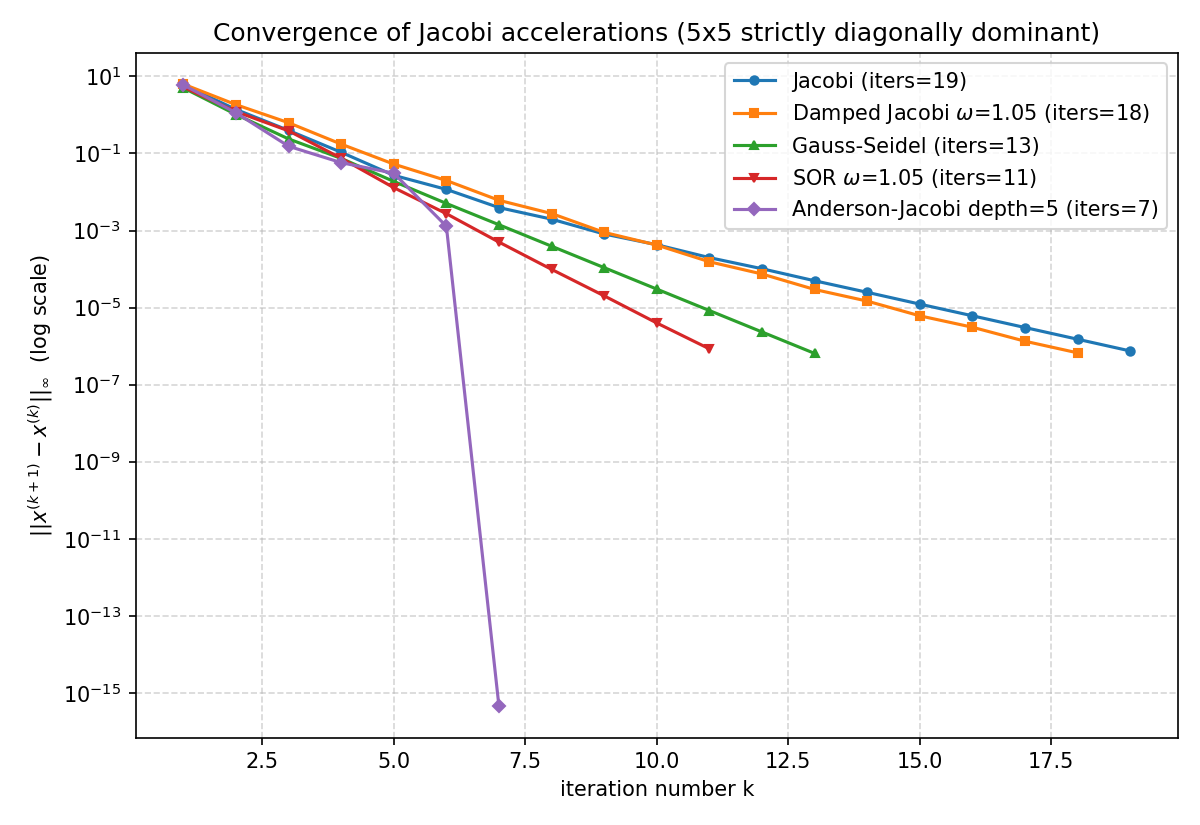
\includegraphics[width=0.82\textwidth]{jacobi_acceleration_comparison.png}
  \caption{四种加速方法与标准雅可比的收敛曲线对比（半对数坐标）}
  \label{fig:accel}
\end{figure}

\begin{figure}[htbp]
  \centering
  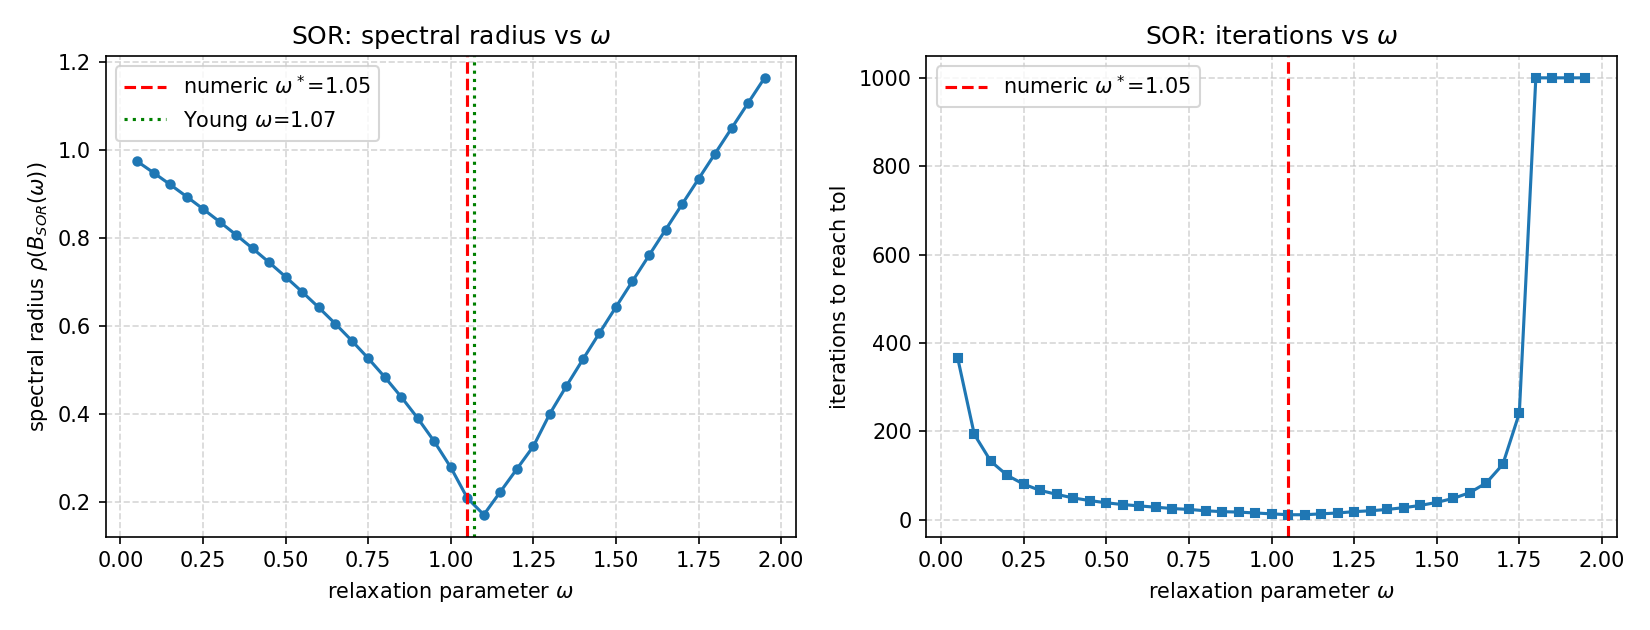
\includegraphics[width=0.92\textwidth]{sor_omega_scan.png}
  \caption{SOR 的谱半径与迭代次数随松弛因子 $\omega$ 的变化}
  \label{fig:sor}
\end{figure}

\subsection{分析与讨论}

\begin{enumerate}
  \item \textbf{高斯--赛德尔优于雅可比。}实验测得 $\rho(B_{GS})\approx0.2777$，
    与 $\rho(B_J)^2\approx0.246$ 同量级，印证了“高斯--赛德尔通常比雅可比收敛更快”
    的经验规律；迭代次数由 $19$ 次降至 $13$ 次。
  \item \textbf{SOR 进一步提速，但提升有限。}数值扫描得到最优松弛因子
    $\omega^{\ast}\approx1.05$，对应 $\rho(B_{SOR})\approx0.2081$，迭代 $11$ 次。
    由 Young 定理给出的解析值 $\omega^{\ast}=2/(1+\sqrt{1-\rho(B_J)^2})\approx
    1.0706$ 与数值结果接近但不完全相同：该公式只在“一致有序”矩阵下严格成立，而
    本实验矩阵是普通稠密矩阵，不满足该前提，故此处采用数值扫描而不误用定理。
  \item \textbf{Anderson 加速效果最显著。}取深度 $m=5$ 时仅 $7$ 次迭代即达机器
    精度（相对误差 $\sim10^{-16}$），与“线性问题的 Anderson 加速等价于 GMRES、
    至多 $n$ 步收敛”的理论一致；深度越大效果越好（$m=1\to13$ 次，$m=5\to7$ 次），
    但单步最小二乘开销也随之增大。
  \item \textbf{诚实的限制。}本实验为 $5\times5$ 小规模稠密矩阵，加速比（最高
    $2.71\times$）远小于 Pratapa 等~\cite{pratapa2015} 在大规模稀疏系统上报告的
    “四个数量级”。小矩阵上直接法本身极快、迭代开销差异不显著；Anderson/SOR 等
    加速方法的真正价值在于大规模稀疏问题，这一点与文献结论一致。
\end{enumerate}

\section{总结}

本实验从零实现了雅可比迭代法（仅用 Python + NumPy 的矩阵运算，未调用
\verb|scipy.linalg| 或 \verb|np.linalg.solve| 来绕过迭代），构造并验证了一个
$5\times5$ 严格对角占优矩阵，完成了迭代求解、收敛曲线绘制以及与直接法的对比。
实验确认：
\begin{itemize}
  \item 严格对角占优矩阵保证 $\rho(B)\le\|B\|_{\infty}<1$，雅可比迭代必收敛；
  \item 本实验 $\rho(B)\approx0.4964$，误差呈一阶线性收敛，$19$ 次迭代后
    $\|x^{(k+1)}-x^{(k)}\|_{\infty}\approx 7.5\times10^{-7}$，达到 $10^{-6}$ 容差；
  \item 迭代解与直接法参考解的相对误差约为 $2.1\times10^{-7}$，二者高度一致；
  \item 加速方法对比中，高斯--赛德尔、SOR（$\omega^{\ast}\approx1.05$）与
    Anderson 加速分别将迭代次数降至 $13$、$11$、$7$ 次，其中 Anderson 加速达到
    机器精度，验证了加速方法的有效性，也说明这些方法的真正价值在于大规模稀疏问题。
\end{itemize}

\begin{thebibliography}{99}

\bibitem{golub2013}
G.~H. Golub and C.~F. Van~Loan, \emph{Matrix Computations}, 4th ed.,
Johns Hopkins University Press, 2013. DOI: \texttt{10.56021/9781421407944}.

\bibitem{saad2003}
Y. Saad, \emph{Iterative Methods for Sparse Linear Systems}, 2nd ed.,
Society for Industrial and Applied Mathematics (SIAM), 2003.
DOI: \texttt{10.1137/1.9780898718003}.

\bibitem{varga2000}
R.~S. Varga, \emph{Matrix Iterative Analysis}, 2nd ed., Springer, 2000.
DOI: \texttt{10.1007/978-3-642-05156-2}.

\bibitem{milaszewicz1987}
J.~P. Milaszewicz, Improving Jacobi and Gauss--Seidel iterations,
\emph{Linear Algebra and its Applications}, 1987.
DOI: \texttt{10.1016/S0024-3795(87)90321-1}.

\bibitem{pratapa2015}
P.~P. Pratapa, P. Suryanarayana, and J.~E. Pask, Anderson acceleration of the
Jacobi iterative method: an efficient alternative to Krylov methods for large,
sparse linear systems, \emph{Journal of Computational Physics}, 2015.
DOI: \texttt{10.1016/j.jcp.2015.11.018}.

\end{thebibliography}

\end{document}

